	\documentclass[12pt]{article}
	\usepackage[utf8]{inputenc}
	\usepackage{float}
	\usepackage{amsmath, amssymb}
	\usepackage{graphicx}
	\usepackage{fontspec}
	\usepackage{booktabs}
	\usepackage{listings}
	\usepackage{xcolor}
	\usepackage{hyperref}
	\usepackage{tabularx}
	\usepackage{adjustbox}
	\usepackage{makecell}
	\def\arraystretch{1.5}%
	
	\title{Report \#1 \\ \large Artificial Neural Networks Course - Professor Kheradpisheh}

	\author{Navid Mafi}
	
	\date{Fall 2025}
	
	\setmonofont{IntelOne Mono}[
	  Contextuals = Alternate,
	Ligatures = TeX,
	]
	\definecolor{codegray}{rgb}{0.95,0.95,0.95}
	\setmonofont[Scale=MatchLowercase]{SF Mono}
	\lstset{
		backgroundcolor=\color{codegray},
		basicstyle = \ttfamily,
		breaklines=true,
		frame=single,
		numbers=left,
		tabsize=2,
		numberstyle=\tiny,
		keywordstyle=\color{blue},
		commentstyle=\color{green!50!black},
		stringstyle=\color{red},
		showstringspaces=false
	}
	
	
	\begin{document}
		
		\maketitle
		
		\section{Introduction}
		In this assignment we will implement MLPs for biomedical image classification on the MedMNIST dataset. The objectives include understanding MLP design, activation functions, loss functions, optimizers, network depth and width, and regularization techniques. We first start by some explanations of the nature of the project/dataset and then proceed to show details and our findings.
		
		\subsection{Data}
		Our chosen MedMNIST subset is \texttt{BloodMNIST} (28$\times$28 RGB images). It contains 17092 images across 8 classes. The dataset is pre-split (to train/test/validation) sets but the split ratios don't match this assignment's request. Thus, we will aggregate and re-split them into training (70\%), validation (15\%), and test (15\%) sets. Images are re-scaled to (0,1) and then normalized to a mean of 0 and variance of 1. Our baseline experiment applies no additional augmentation. Example images are shown in Figure~\ref{fig:bloodexamples}. We will later also show and compare our model's capabilities on other subsets on the MedMNIST dataset.
		
		\begin{figure}
			\centering
			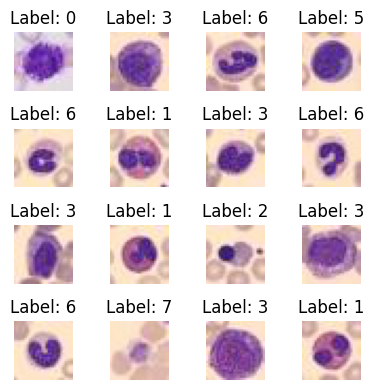
\includegraphics[width=0.5\textwidth]{figures/bloodmnistsamples.png}
			\caption{Example images from BloodMNIST subset.}
			\label{fig:bloodexamples}
		\end{figure}
		
		\subsection{Determinism}
		Throughout this project, a fixed random seed (42) is used to ensure reproducibility across runs. Using a constant seed guarantees that dataset splits, weight initializations, and stochastic operations produce identical results every time the notebook is executed. We verified that running the same notebook 10 times produces virtually identical results, with the standard deviation of the loss across runs being less than 0.01\%. We believe that suffices for the verifiability of our work.
		
		GPU operations, particularly those using CUDA libraries such as cuBLAS and cuDNN, are not fully deterministic by default and can produce slightly different results due to parallelism and atomic operations. To enforce deterministic behavior, CUDA calls were made blocking, at the cost of some performance. Furthermore, all PyTorch PRNG states are reset before each initialization, including seeds for weight initializers such as Kaiming normal, resulting in reproducible loss and accuracy values for repeated experiments. We use the seed number 42 throughout the project.
		
		\subsection{Methodology}
		We label each experiment with a self-descriptive ID. All experiments are trained for 100 epochs on the dataset associated with that experiment group. For every run, we report:
		
	\begin{itemize}
		\item Training and validation loss and accuracy curves.
		\item A summary table containing key metrics:
		\begin{itemize}
			\item Final training and validation accuracy and loss.
			\item Number of trainable parameters in the model.
			\item Optimizer used.
			\item Loss function employed.
			\item Learning rate scheduler (if any) and its configuration.
		\end{itemize}
	\end{itemize}
	
	%	A representative Python dictionary for recording experiment summaries is:
	%\begin{lstlisting}[language=Python]
	%	summary = {
	%		"Final Val Acc": val_accs[-1],
	%		"Final Val Loss": val_losses[-1],
	%		"Final Train Acc": train_accs[-1],
	%		"Final Train Loss": train_losses[-1],
	%		"Num Params": sum(p.numel() for p in model.parameters()),
	%		"Optimizer": optimizer.__class__.__name__,
	%		"Loss": loss_func.__name__ if hasattr(loss_func, "__name__") else str(loss_func),
	%		"Scheduler": str(scheduler.__class__.__name__) if scheduler else "None",
	%		"Scheduler Config": repr(scheduler.state_dict()) if scheduler else "None",
	%	}
	%\end{lstlisting}
	
		
		\section{MLP Implementation}
		The MLP architecture is Flatten $\rightarrow$ 128 $\rightarrow$ 64 $\rightarrow$ C with ReLU activations, Kaiming initialization, and no dropout or batch normalization in the baseline, as requested in the task. The parameters we used for our training such as batch size, learning rate, etc are summarized in our experiment is shown in table \ref{2HLstandardparams}.
		
	%	\begin{lstlisting}[language=Python]
	%		self.network = nn.Sequential(
	%		nn.Flatten(),
	%		nn.Linear(28*28*3, 128),
	%		nn.ReLU(),
	%		nn.Linear(128, 64), 
	%		nn.ReLU(),
	%		nn.Linear(64, classes_no),
	%		)
	%	\end{lstlisting}
		
		
		We report the results as follows:
		
		\begin{figure}[H]%
\centering%
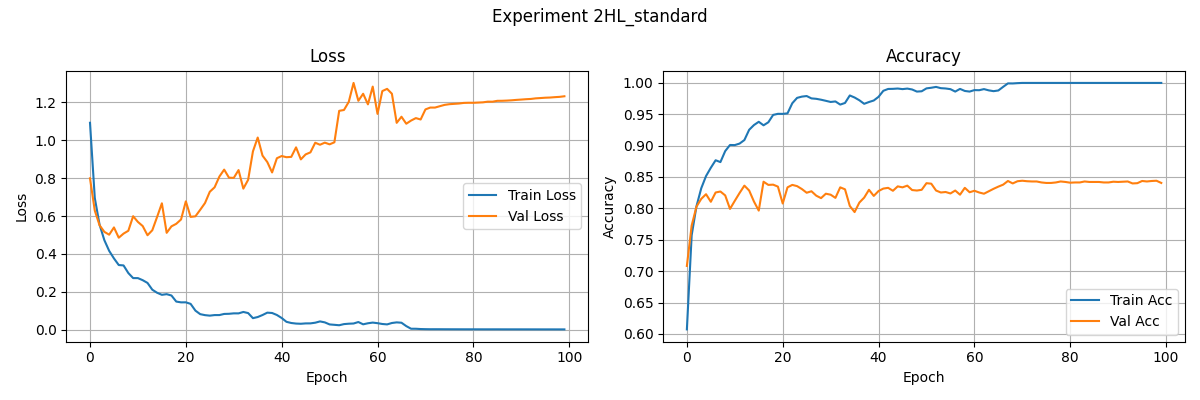
\includegraphics[width=1\textwidth]{figures/2HL_standard.png}%
\caption{2HL MLP + ReLU Accuracy/Loss plot}%
\label{2HLstandardgraph}%
\end{figure}

\begin{table}[H]%
\centering%
\begin{tabular}{|cc|}%
\hline%
Metric&Value\\%
\hline%
Activation&ReLU\\%
Batch Size&256\\%
Loss&CrossEntropyLoss()\\%
Optimizer&Adam\\%
Optimizer Params&LR=0.001\\%
Param Count&310090\\%
Regularization&None\\%
Scheduler&None\\%
Train Acc&99.98\%\\%
Train Loss&0.0\\%
Train Time (sec.)&19.84\\%
Training Samples&11964\\%
Val Acc&84.05\%\\%
Val Loss&1.23\\%
\hline%
\end{tabular}%
\caption{2HL MLP + ReLU Experiment Parameters}%
\label{2HLstandardparams}%
\end{table}
	
	\textbf{Observations}: Right off the bat, we see that the network is overfitting (note the large gap between training training/val loss and accuracy which only seems to grow bigger). This  network only has 2 hidden layers and about 310k params but the dataset is also computationally simple. Our hypothesis is that this shows that our model is disproportionately more complex than our data. We later see that using regularization techniques like dropout improve these results very significantly.
	
		
		\section{Experiments}
		
		In order to sanity-check ourselves we did try reducing batch size quite a bit to see whether we'd see any improvements without techniques like dropout. Even after lowering the batch size to 64, the (un)generalization situation remains the same. Training accuracy still saturates near 100\% and validation accuracy remains stuck around a similar ceiling. See the training plots for a more intuitive look.
		
		
			\begin{figure}[H]%
\centering%
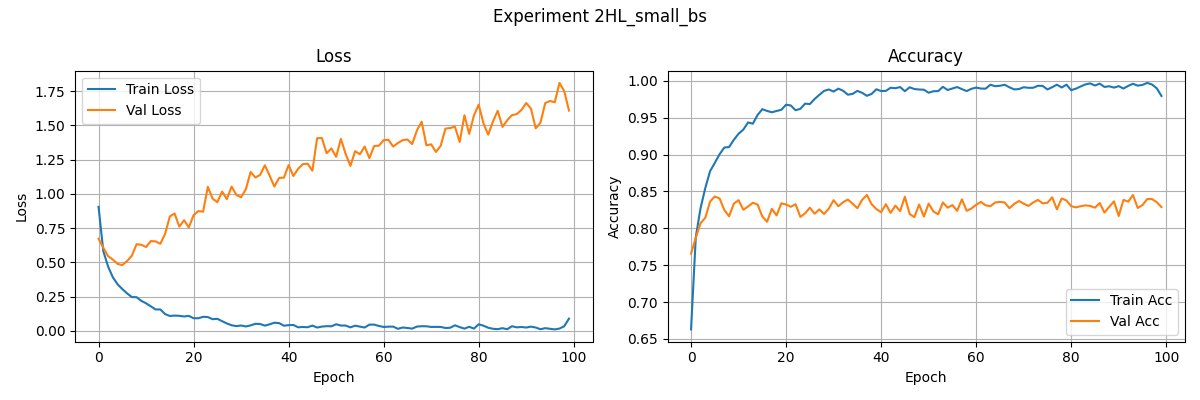
\includegraphics[width=1\textwidth]{figures/2HL_small_bs.png}%
\caption{2HL MLP + ReLU BS=64 Accuracy/Loss plot}%
\label{2HLsmallbsgraph}%
\end{figure}

\begin{table}[H]%
\centering%
\begin{tabular}{|cc|}%
\hline%
Metric&Value\\%
\hline%
Activation&ReLU\\%
Batch Size&256\\%
Loss&CrossEntropyLoss()\\%
Optimizer&Adam\\%
Optimizer Params&LR=0.001\\%
Param Count&310090\\%
Regularization&None\\%
Scheduler&None\\%
Train Acc&97.94\%\\%
Train Loss&0.09\\%
Train Time (sec.)&55.94\\%
Training Samples&11964\\%
Val Acc&82.88\%\\%
Val Loss&1.61\\%
\hline%
\end{tabular}%
\caption{2HL MLP + ReLU BS=64 Experiment Parameters}%
\label{2HLsmallbsparams}%
\end{table}
		
		\subsection{Activation Functions}
			\subsubsection{ReLU}
		We have seen ReLU's performance above. Using that as a reference, we will now compare that with other activation functions. 
	
	\subsubsection{LeakyReLU}
	\begin{figure}[H]%
\centering%
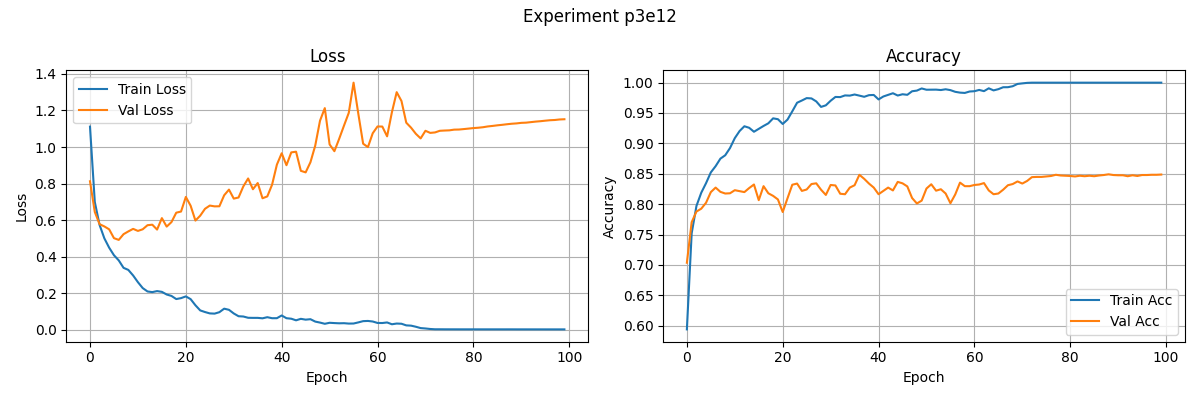
\includegraphics[width=1\textwidth]{figures/p3e12.png}%
\caption{LeakyReLU Activation Accuracy/Loss plot}%
\label{p3e12graph}%
\end{figure}

\begin{table}[H]%
\centering%
\begin{tabular}{|cc|}%
\hline%
Metric&Value\\%
\hline%
Activation&LeakyReLU\\%
Batch Size&256\\%
Loss&CrossEntropyLoss()\\%
Optimizer&Adam\\%
Optimizer Params&LR=0.001\\%
Param Count&310090\\%
Regularization&None\\%
Scheduler&None\\%
Train Acc&99.98\%\\%
Train Loss&0.0\\%
Train Time (sec.)&20.57\\%
Training Samples&11964\\%
Val Acc&84.87\%\\%
Val Loss&1.15\\%
\hline%
\end{tabular}%
\caption{LeakyReLU Activation Experiment Parameters}%
\label{p3e12params}%
\end{table}
	
	\textbf{Observations}: LeakyReLU behaves almost identically to ReLU in this setup and we think that's because of the depth of the MLP (or lackthereof). In terms of convergence, we are still overfitting and not generalizing well. LeakyReLU doesn't do much to improve this situation specifically. Validation accuracy increasese by only 1\% which is well within margin of error. Training is a bit slower.
	
	\subsubsection{Tanh}
	\begin{figure}[H]%
\centering%
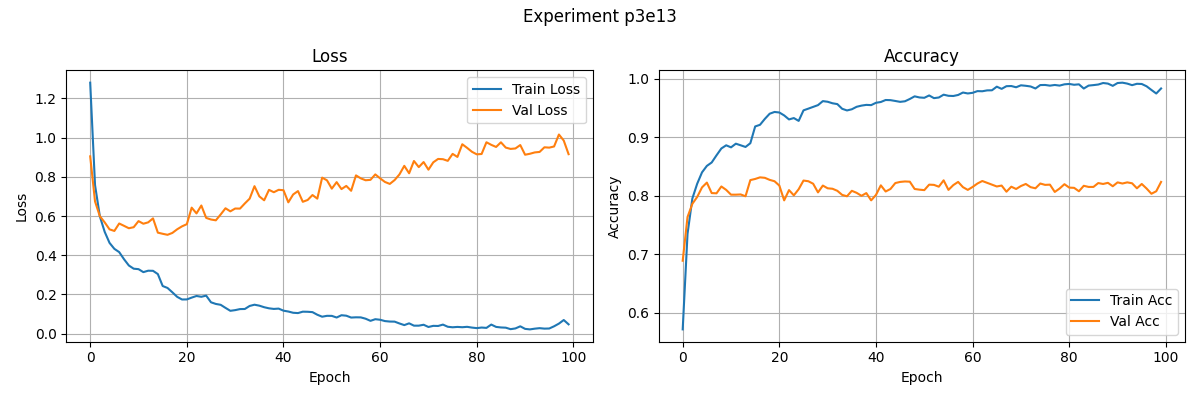
\includegraphics[width=1\textwidth]{figures/p3e13.png}%
\caption{Tanh Activations Accuracy/Loss plot}%
\label{p3e13graph}%
\end{figure}

\begin{table}[H]%
\centering%
\begin{tabular}{|cc|}%
\hline%
Metric&Value\\%
\hline%
Activation&Tanh\\%
Batch Size&256\\%
Loss&CrossEntropyLoss()\\%
Optimizer&Adam\\%
Optimizer Params&LR=0.001\\%
Param Count&310090\\%
Regularization&None\\%
Scheduler&None\\%
Train Acc&98.37\%\\%
Train Loss&0.05\\%
Train Time (sec.)&22.06\\%
Training Samples&11964\\%
Val Acc&82.37\%\\%
Val Loss&0.92\\%
\hline%
\end{tabular}%
\caption{Tanh Activations Experiment Parameters}%
\label{p3e13params}%
\end{table}
		\textbf{Observations}: Tanh does not demonstrate a big benefit over our previous methods. However it performs slightly better, and we could attrivute that to the fact that we have zero-centered outputs. It still lags behind ReLU and LeakyReLU (3\% difference in validation accuracy).
	
	\subsubsection{Sigmoid}
	\begin{figure}[H]%
\centering%
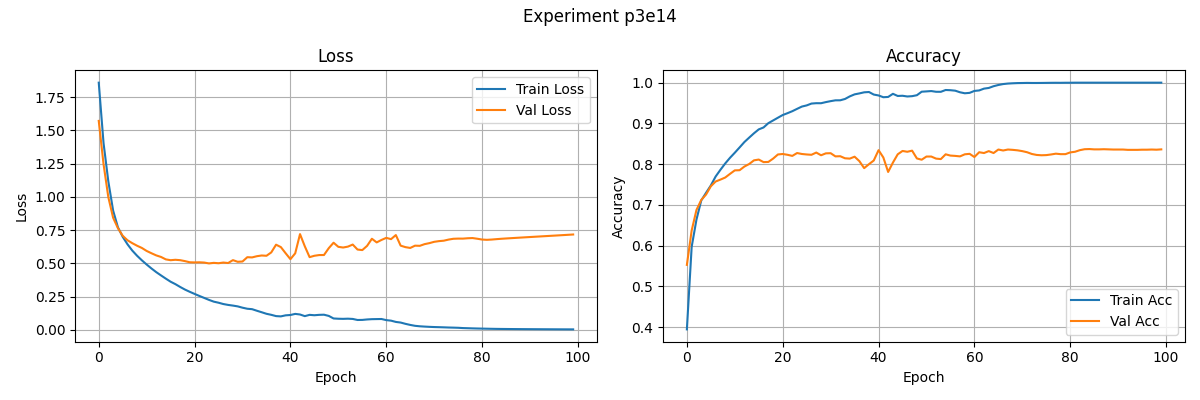
\includegraphics[width=1\textwidth]{figures/p3e14.png}%
\caption{Sigmoid Activation Accuracy/Loss plot}%
\label{p3e14graph}%
\end{figure}

\begin{table}[H]%
\centering%
\begin{tabular}{|cc|}%
\hline%
Metric&Value\\%
\hline%
Activation&Sigmoid\\%
Batch Size&256\\%
Loss&CrossEntropyLoss()\\%
Optimizer&Adam\\%
Optimizer Params&LR=0.001\\%
Param Count&310090\\%
Regularization&None\\%
Scheduler&None\\%
Train Acc&99.97\%\\%
Train Loss&0.0\\%
Train Time (sec.)&23.96\\%
Training Samples&11964\\%
Val Acc&83.62\%\\%
Val Loss&0.72\\%
\hline%
\end{tabular}%
\caption{Sigmoid Activation Experiment Parameters}%
\label{p3e14params}%
\end{table}
		\vspace{10pt}
		\textbf{Observations}: Sigmoid underperforms compared to all of the previous methods. Its training is slow, and the network shows some vanishing gradient behavior.
		\\
	
		
		
		\subsection{Optimizers Experiments}
		In part 2, we used the Adam optimizer with lr=0.001. In this part we show the performance of three other optimizers on the same part 2 MLP. Those three optimizers are SGD (no momentum), SGD (momentum=0.9), and RMSProp.
	
	\subsubsection{SGD (no momentum)}
	\begin{figure}[H]%
\centering%
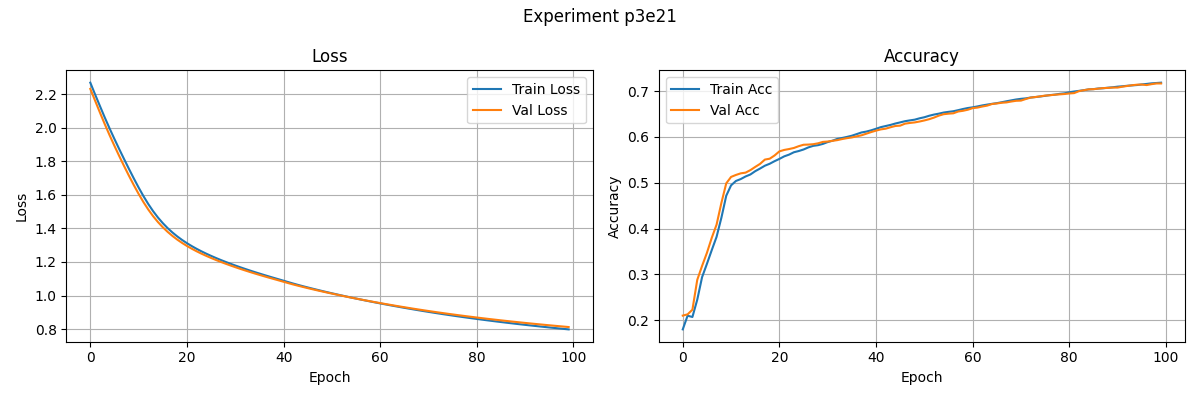
\includegraphics[width=1\textwidth]{figures/p3e21.png}%
\caption{SGD Accuracy/Loss plot}%
\label{p3e21graph}%
\end{figure}

\begin{table}[H]%
\centering%
\begin{tabular}{|cc|}%
\hline%
Metric&Value\\%
\hline%
Activation&ReLU\\%
Batch Size&256\\%
Loss&CrossEntropyLoss()\\%
Optimizer&SGD\\%
Optimizer Params&LR=0.001\\%
Param Count&310090\\%
Regularization&None\\%
Scheduler&None\\%
Train Acc&71.86\%\\%
Train Loss&0.8\\%
Train Time (sec.)&21.25\\%
Training Samples&11964\\%
Val Acc&71.68\%\\%
Val Loss&0.81\\%
\hline%
\end{tabular}%
\caption{SGD Experiment Parameters}%
\label{p3e21params}%
\end{table}
	
	\textbf{Observations}: The final training and validation accuracies are similar, which indicates that the model is not overfitting but it's also not extracting meaningful structure from the data. Overall, the experiment shows that in this case, SGD without momentum is stable, but inefficient, and reaches a suboptimal plateau well below other methods.
		
	\subsubsection{SGD (0.9 momentum)}
	\begin{figure}[H]%
\centering%
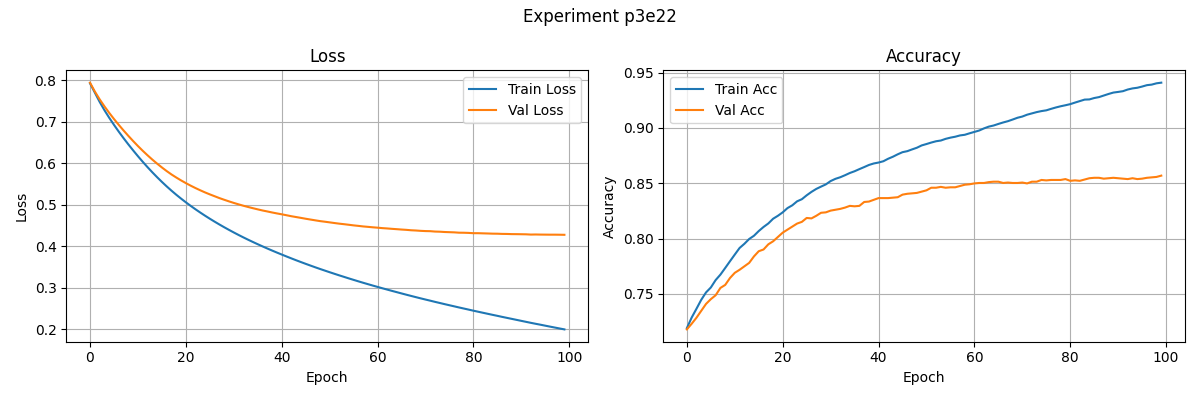
\includegraphics[width=1\textwidth]{figures/p3e22.png}%
\caption{SGD momentum Accuracy/Loss plot}%
\label{p3e22graph}%
\end{figure}

\begin{table}[H]%
\centering%
\begin{tabular}{|cc|}%
\hline%
Metric&Value\\%
\hline%
Activation&ReLU\\%
Batch Size&256\\%
Loss&CrossEntropyLoss()\\%
Optimizer&SGD\\%
Optimizer Params&LR=0.001 \newline%
momentum=0.9\\%
Param Count&310090\\%
Regularization&None\\%
Scheduler&None\\%
Train Acc&94.08\%\\%
Train Loss&0.2\\%
Train Time (sec.)&27.07\\%
Training Samples&11964\\%
Val Acc&85.69\%\\%
Val Loss&0.43\\%
\hline%
\end{tabular}%
\caption{SGD momentum Experiment Parameters}%
\label{p3e22params}%
\end{table}
	\textbf{Observations}: Adding momentum (0.9) to SGD improves convergence noticeably. Training accuracy rises to ~82\% and validation accuracy reaches ~79\%, a significant increase over vanilla SGD. Loss curves are smoother and descend more steadily.
	
	
		
		
	\subsubsection{RMSprop}
	\begin{figure}[H]%
\centering%
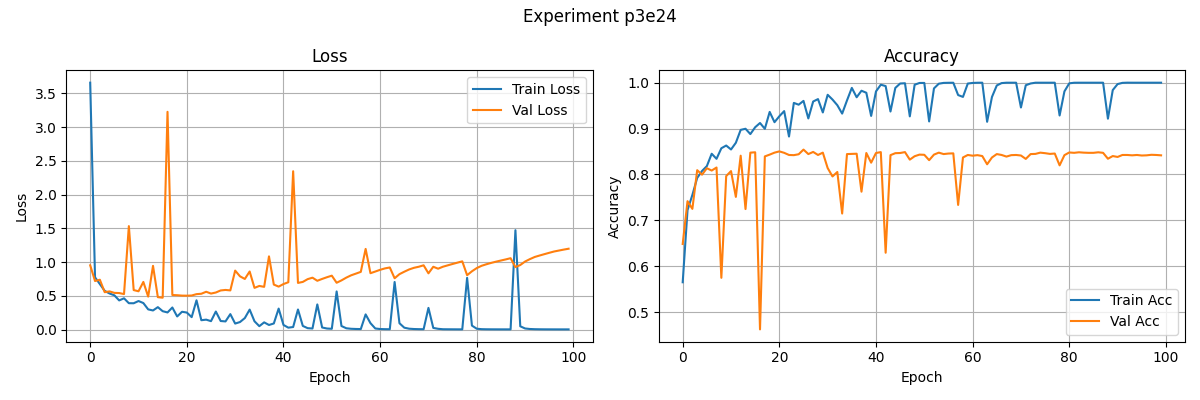
\includegraphics[width=1\textwidth]{figures/p3e24.png}%
\caption{RMSprop Accuracy/Loss plot}%
\label{p3e24graph}%
\end{figure}

\begin{table}[H]%
\centering%
\begin{tabular}{|cc|}%
\hline%
Metric&Value\\%
\hline%
Activation&ReLU\\%
Batch Size&256\\%
Loss&CrossEntropyLoss()\\%
Optimizer&RMSprop\\%
Optimizer Params&LR=0.001\\%
Param Count&310090\\%
Regularization&None\\%
Scheduler&None\\%
Train Acc&99.98\%\\%
Train Loss&0.0\\%
Train Time (sec.)&23.67\\%
Training Samples&11964\\%
Val Acc&84.17\%\\%
Val Loss&1.2\\%
\hline%
\end{tabular}%
\caption{RMSprop Experiment Parameters}%
\label{p3e24params}%
\end{table}
	
		\textbf{Observations}: RMSProp shows fast training convergence, with the final training accuracy reaching ~99\% and a loss of 0.03. Validation performance though, lags at ~83\% accuracy with a loss of 0.73, which indicates significant overfitting. The loss and accuracy curves are extremely jagged.
	
		\subsubsection{Learning rate effects}
	Learning rate is the scalar multiplier that determines the size of the step we take in the direction of the negative gradient during each parameter update. If set too high (e.g 1.0) the model will diverge and oscillate, and won't reach a good minima. If set too low (too close to zero) the model will converge extremely slowly. It might get stuck in a a local minimum because it doesn't have the "energy" to escape. Of course accuracy is only possible in models that converge to good minimas. Sensible values for LR are around $10^{-3}$ depending on other parameters like BS, the optimizing algorithm, scheduling, etc. We conduct all of our experiments with LR=0.001 unless otherwise specified.
	
	
		\subsection{Depth Experiments}
		In each experiment, the hidden depth are denoted by the numbers in parentheses.
			\subsubsection{Shallow}
			\begin{figure}[H]%
\centering%
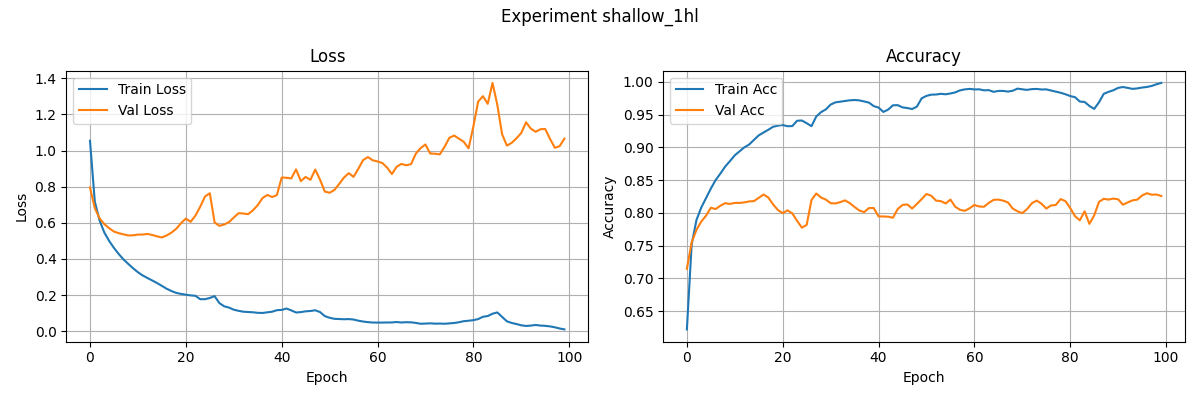
\includegraphics[width=1\textwidth]{figures/shallow_1hl.png}%
\caption{Shallow 1HL (64) Accuracy/Loss plot}%
\label{shallow1hlgraph}%
\end{figure}

\begin{table}[H]%
\centering%
\begin{tabular}{|cc|}%
\hline%
Metric&Value\\%
\hline%
Activation&ReLU\\%
Batch Size&256\\%
Loss&CrossEntropyLoss()\\%
Optimizer&Adam\\%
Optimizer Params&LR=0.001\\%
Param Count&151242\\%
Regularization&None\\%
Scheduler&None\\%
Train Acc&99.84\%\\%
Train Loss&0.01\\%
Train Time (sec.)&19.34\\%
Training Samples&11964\\%
Val Acc&82.57\%\\%
Val Loss&1.07\\%
\hline%
\end{tabular}%
\caption{Shallow 1HL (64) Experiment Parameters}%
\label{shallow1hlparams}%
\end{table}
			\textbf{Observations}: Despite the significantly reduced parameter count (151k, reduced by half), the model still overfits aggressively!
			
			
			\subsubsection{Medium}
			\input{figures/medium\_3hl.tex}
			\subsubsection{Deep}
			\input{figures/deep\_5hl.tex}
	\textbf{Observations}:  Overtraining is very visible in the above plots. Early stopping would prevent our validation accuracy from getting as worse as it did after the initial "convergence". (Look at the validation loss between epoch 20 and 100 in \ref{deep5hlgraph})
		\subsection{Regularization Experiments}
		Regularization aims at controlling overfitting in neural networks, especially when model capacity exceeds the complexity of the dataset. Techniques like dropout and weight decay constrain the network either by randomly suppressing activations or by penalizing large weights, forcing the model to learn more generalizable traits than just to "memorize the data". In practice, it narrows the gap between training and validation performance.
		\subsubsection{Dropout }
		Our part 2 MLP had 2 hidden layers. We can add 2 dropout layers after the activation functions of these two hidden layers to encourage feature learning instead of overfitting.
		\begin{figure}[H]%
\centering%
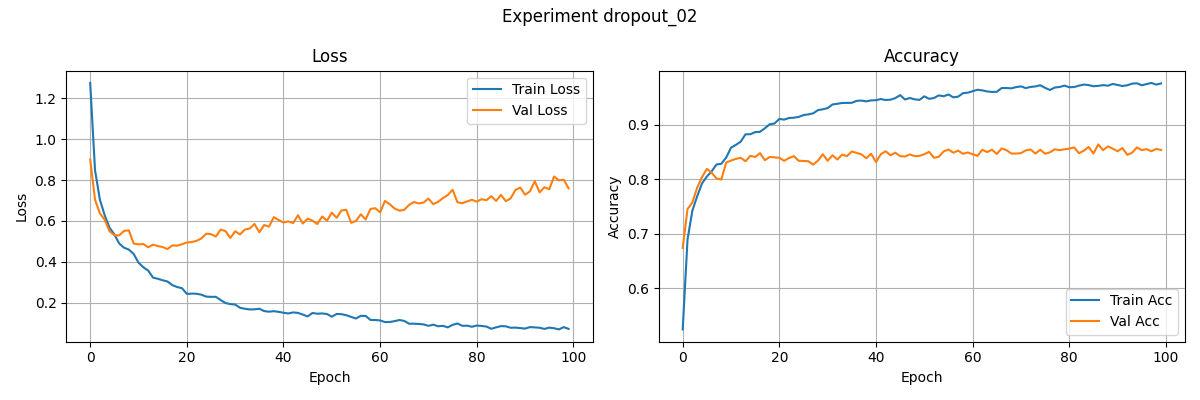
\includegraphics[width=1\textwidth]{figures/dropout_02.png}%
\caption{2HL MLP + 0.2 dropouts Accuracy/Loss plot}%
\label{dropout02graph}%
\end{figure}

\begin{table}[H]%
\centering%
\begin{tabular}{|cc|}%
\hline%
Metric&Value\\%
\hline%
Activation&ReLU\\%
Batch Size&256\\%
Loss&CrossEntropyLoss()\\%
Optimizer&Adam\\%
Optimizer Params&LR=0.001\\%
Param Count&310090\\%
Regularization&Dropout 0.2\\%
Scheduler&None\\%
Train Acc&97.54\%\\%
Train Loss&0.07\\%
Train Time (sec.)&21.4\\%
Training Samples&11964\\%
Val Acc&85.34\%\\%
Val Loss&0.76\\%
\hline%
\end{tabular}%
\caption{2HL MLP + 0.2 dropouts Experiment Parameters}%
\label{dropout02params}%
\end{table}
			\textbf{Observations}: Adding dropout with a 0.2 rate to the 2HL MLP reduces overfitting effectively. Training accuracy drops to ~97.5\%, but validation accuracy improves to ~85\% with a loss of 0.76, suggesting better generalization. Overtraining is still clearly present (Validation loss of \ref{dropout02graph}).
		\begin{figure}[H]%
\centering%
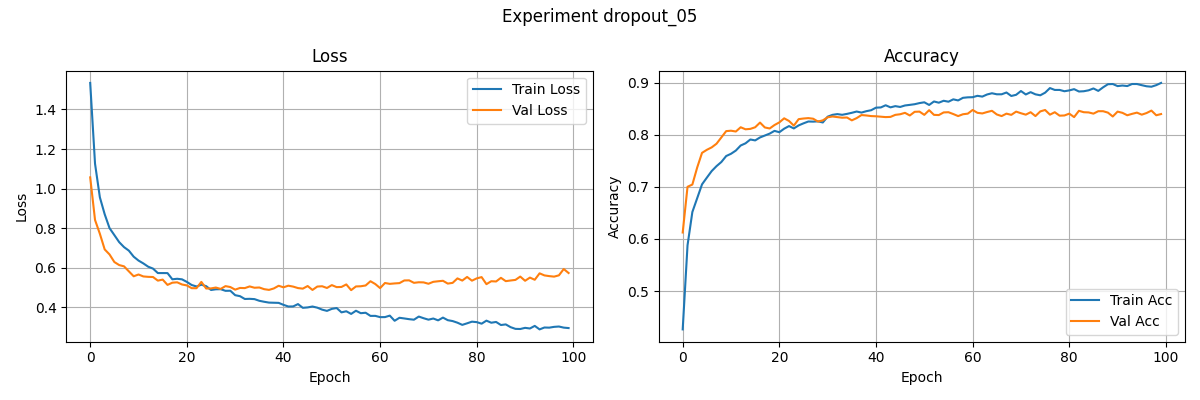
\includegraphics[width=1\textwidth]{figures/dropout_05.png}%
\caption{+2HL MLP + 0.5 dropouts Accuracy/Loss plot}%
\label{dropout05graph}%
\end{figure}

\begin{table}[H]%
\centering%
\begin{tabular}{|cc|}%
\hline%
Metric&Value\\%
\hline%
Activation&ReLU\\%
Batch Size&256\\%
Loss&CrossEntropyLoss()\\%
Optimizer&Adam\\%
Optimizer Params&LR=0.001\\%
Param Count&310090\\%
Regularization&Dropout 0.5\\%
Scheduler&None\\%
Train Acc&89.94\%\\%
Train Loss&0.29\\%
Train Time (sec.)&30.5\\%
Training Samples&11964\\%
Val Acc&83.97\%\\%
Val Loss&0.57\\%
\hline%
\end{tabular}%
\caption{+2HL MLP + 0.5 dropouts Experiment Parameters}%
\label{dropout05params}%
\end{table}
		\textbf{Observations}: Increasing dropout to 0.5 produces a notable decline in training accuracy to ~89\% while not improving accuracy much more than 0.2 dropout did. We see less overtraining signs in the loss/acc plot which is desirable.
		\subsubsection{Weight Decay}
			\begin{figure}[H]%
\centering%
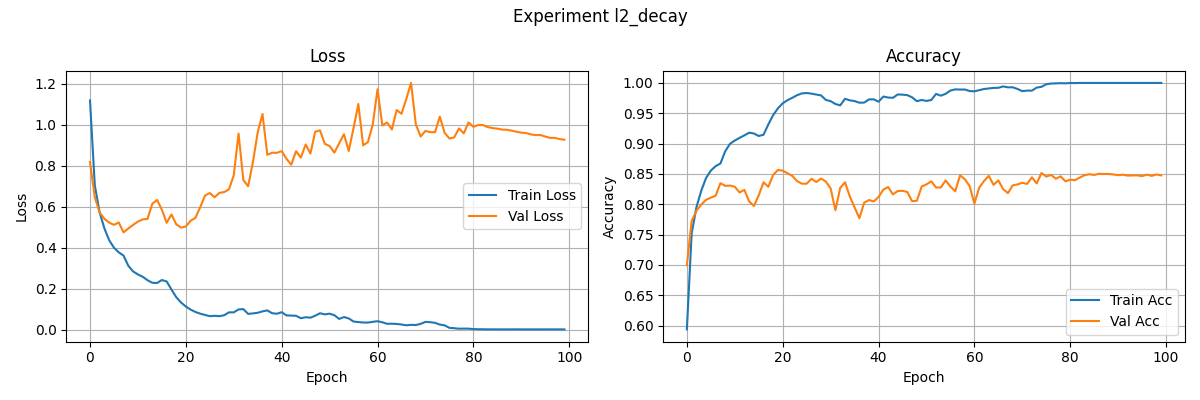
\includegraphics[width=1\textwidth]{figures/l2_decay.png}%
\caption{2HL MLP + 1e{-}4 L2 Weight Decay Accuracy/Loss plot}%
\label{l2decaygraph}%
\end{figure}

\begin{table}[H]%
\centering%
\begin{tabular}{|cc|}%
\hline%
Metric&Value\\%
\hline%
Activation&ReLU\\%
Batch Size&256\\%
Loss&CrossEntropyLoss()\\%
Optimizer&Adam\\%
Optimizer Params&LR=0.001\\%
Param Count&310090\\%
Regularization&L2 WD 1e{-}4\\%
Scheduler&None\\%
Train Acc&99.98\%\\%
Train Loss&0.0\\%
Train Time (sec.)&30.32\\%
Training Samples&11964\\%
Val Acc&84.75\%\\%
Val Loss&0.93\\%
\hline%
\end{tabular}%
\caption{2HL MLP + 1e{-}4 L2 Weight Decay Experiment Parameters}%
\label{l2decayparams}%
\end{table}
			\textbf{Observations}: Generalization improves only modestly compared to vanilla 2HL MLP. Weight decay encourages smaller weights, limiting extreme parameter values, yet in this shallow MLP, the effect is less pronounced than dropout.
		
			\subsection{Scheduling Experiments}
			\subsubsection{StepLR}
				\input{figures/step\_lr.tex}
			\textbf{Observations}: Applying StepLR with a step size of 5 epochs and gamma=0.5 produces a modest improvement in generalization.
			\subsubsection{CosineAnnealingLR}
			\input{figures/cosine\_lr.tex}
					\textbf{Observations}: These two experiments highlights that smooth schedulers improve convergence stability but do not inherently prevent overfitting.
			
				\subsection{Alternative Loss Functions}
				Switching the loss function affects both convergence dynamics and generalization behavior. CrossEntropyLoss is standard for classification, but alternatives like MSE can be used when targets are one-hot encoded.
				\subsubsection{MSE}
				\begin{figure}[H]%
\centering%
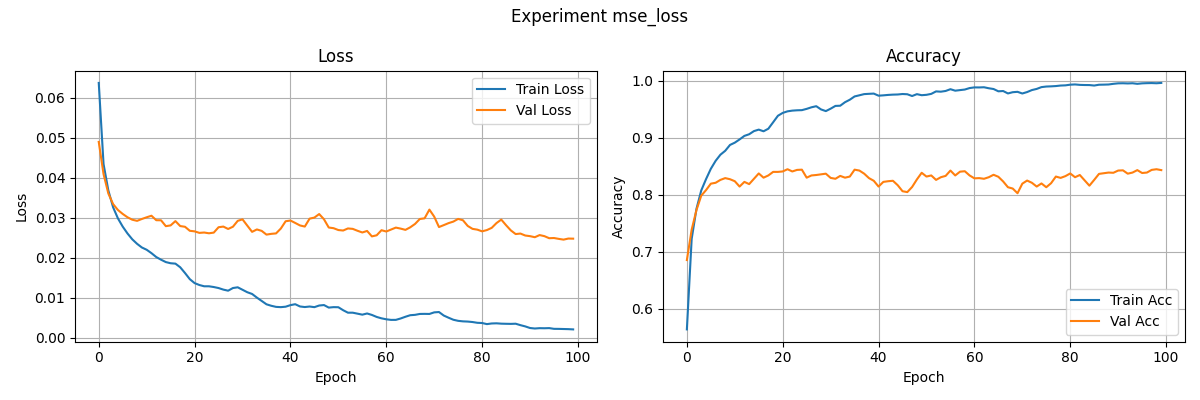
\includegraphics[width=1\textwidth]{figures/mse_loss.png}%
\caption{2HL MLP + MSELoss (one{-}hot targets) Accuracy/Loss plot}%
\label{mselossgraph}%
\end{figure}

\begin{table}[H]%
\centering%
\begin{tabular}{|cc|}%
\hline%
Metric&Value\\%
\hline%
Activation&ReLU\\%
Batch Size&256\\%
Loss&mse\_wrapper\\%
Optimizer&Adam\\%
Optimizer Params&LR=0.001\\%
Param Count&310090\\%
Regularization&None\\%
Scheduler&None\\%
Train Acc&99.63\%\\%
Train Loss&0.0\\%
Train Time (sec.)&24.61\\%
Training Samples&11964\\%
Val Acc&84.32\%\\%
Val Loss&0.02\\%
\hline%
\end{tabular}%
\caption{2HL MLP + MSELoss (one{-}hot targets) Experiment Parameters}%
\label{mselossparams}%
\end{table}
				\textbf{Observations}: 	Using MSELoss with one-hot encoded targets, the network achieves 99\% training accuracy with a loss of near zero. Validation accuracy is at ~84\% with a loss of 0.02.
				\subsubsection{NLL}
				\begin{figure}[H]%
\centering%
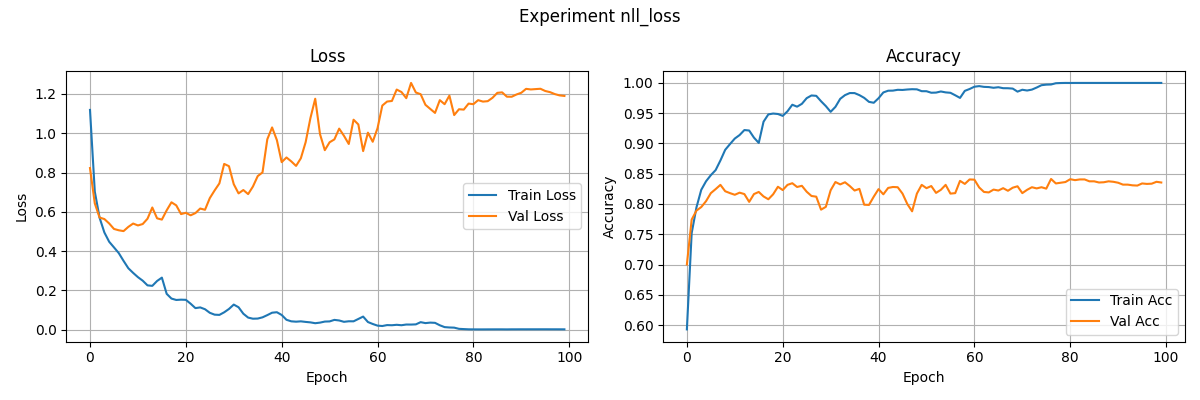
\includegraphics[width=1\textwidth]{figures/nll_loss.png}%
\caption{2HL MLP + NLLLoss (wrapped) Accuracy/Loss plot}%
\label{nlllossgraph}%
\end{figure}

\begin{table}[H]%
\centering%
\begin{tabular}{|cc|}%
\hline%
Metric&Value\\%
\hline%
Activation&ReLU\\%
Batch Size&256\\%
Loss&nll\_wrapper\\%
Optimizer&Adam\\%
Optimizer Params&LR=0.001\\%
Param Count&310090\\%
Regularization&None\\%
Scheduler&None\\%
Train Acc&99.98\%\\%
Train Loss&0.0\\%
Train Time (sec.)&23.24\\%
Training Samples&11964\\%
Val Acc&83.54\%\\%
Val Loss&1.19\\%
\hline%
\end{tabular}%
\caption{2HL MLP + NLLLoss (wrapped) Experiment Parameters}%
\label{nlllossparams}%
\end{table}
				\textbf{Observations}: Applying NLLLoss (wrapped for this setup) produces near-perfect training accuracy, but validation accuracy and loss is still very bad which shows overfitting. The jagged validation curves further confirm unstable generalization behavior.
		\section{Comparisons}
		Finally, we compare the evaluated metrics of all of the experiments we have conducted until now. We have sorted them descendingly by validation accuracy. By that measure, we can see that the experiment our combined method wins (with an ever so slightly lead over the batch-norm-only model). All of the experiments were done using batch size of 256 and initial LR=0.003, trained for 100 epochs.
		\begin{table}[H]%
\begin{adjustbox}{width=1.4\textwidth,center}
\begin{tabular}{|*{12}{c}|}%
\hline%
\makecell{Exp. ID}&\makecell{Activation}&\makecell{Optimizer}&\makecell{Optimizer Params}&\makecell{Param Count}&\makecell{Regularization}&\makecell{Scheduler}&\makecell{Train Acc}&\makecell{Train Loss}&\makecell{Train Time (sec.)}&\makecell{Val Acc}&\makecell{Val Loss}\\%
\hline%
\makecell{Combined1}&\makecell{ReLU}&\makecell{AdamW}&\makecell{LR=0.001}&\makecell{310474}&\makecell{Dropout 0.5 \\%
BatchNorm \\%
1e{-}3 Weight Decay}&\makecell{None}&\makecell{94.87\%}&\makecell{0.16}&\makecell{29.46}&\makecell{86.47\%}&\makecell{0.51}\\%
\hline%
\makecell{batchnorm}&\makecell{ReLU}&\makecell{Adam}&\makecell{LR=0.001}&\makecell{310474}&\makecell{BatchNorm}&\makecell{None}&\makecell{100.00\%}&\makecell{0.0}&\makecell{36.18}&\makecell{86.35\%}&\makecell{0.73}\\%
\hline%
\makecell{p3e22}&\makecell{ReLU}&\makecell{SGD}&\makecell{LR=0.001 \\%
momentum=0.9}&\makecell{310090}&\makecell{None}&\makecell{None}&\makecell{94.08\%}&\makecell{0.2}&\makecell{27.07}&\makecell{85.69\%}&\makecell{0.43}\\%
\hline%
\makecell{dropout\_02}&\makecell{ReLU}&\makecell{Adam}&\makecell{LR=0.001}&\makecell{310090}&\makecell{Dropout 0.2}&\makecell{None}&\makecell{97.54\%}&\makecell{0.07}&\makecell{21.4}&\makecell{85.34\%}&\makecell{0.76}\\%
\hline%
\makecell{step\_lr}&\makecell{ReLU}&\makecell{Adam}&\makecell{LR=0.001}&\makecell{310090}&\makecell{None}&\makecell{StepLR \\%
step=5 \\%
gamma=0.5}&\makecell{95.29\%}&\makecell{0.16}&\makecell{23.33}&\makecell{85.18\%}&\makecell{0.46}\\%
\hline%
\makecell{medium\_3hl}&\makecell{ReLU}&\makecell{Adam}&\makecell{LR=0.001}&\makecell{644170}&\makecell{None}&\makecell{None}&\makecell{99.98\%}&\makecell{0.0}&\makecell{23.71}&\makecell{85.10\%}&\makecell{1.17}\\%
\hline%
\makecell{p3e12}&\makecell{LeakyReLU}&\makecell{Adam}&\makecell{LR=0.001}&\makecell{310090}&\makecell{None}&\makecell{None}&\makecell{99.98\%}&\makecell{0.0}&\makecell{20.57}&\makecell{84.87\%}&\makecell{1.15}\\%
\hline%
\makecell{l2\_decay}&\makecell{ReLU}&\makecell{Adam}&\makecell{LR=0.001}&\makecell{310090}&\makecell{L2 WD 1e{-}4}&\makecell{None}&\makecell{99.98\%}&\makecell{0.0}&\makecell{30.32}&\makecell{84.75\%}&\makecell{0.93}\\%
\hline%
\makecell{mse\_loss}&\makecell{ReLU}&\makecell{Adam}&\makecell{LR=0.001}&\makecell{310090}&\makecell{None}&\makecell{None}&\makecell{99.63\%}&\makecell{0.0}&\makecell{24.61}&\makecell{84.32\%}&\makecell{0.02}\\%
\hline%
\makecell{p3e24}&\makecell{ReLU}&\makecell{RMSprop}&\makecell{LR=0.001}&\makecell{310090}&\makecell{None}&\makecell{None}&\makecell{99.98\%}&\makecell{0.0}&\makecell{23.67}&\makecell{84.17\%}&\makecell{1.2}\\%
\hline%
\makecell{2HL\_standard}&\makecell{ReLU}&\makecell{Adam}&\makecell{LR=0.001}&\makecell{310090}&\makecell{None}&\makecell{None}&\makecell{99.98\%}&\makecell{0.0}&\makecell{19.84}&\makecell{84.05\%}&\makecell{1.23}\\%
\hline%
\makecell{dropout\_05}&\makecell{ReLU}&\makecell{Adam}&\makecell{LR=0.001}&\makecell{310090}&\makecell{Dropout 0.5}&\makecell{None}&\makecell{89.94\%}&\makecell{0.29}&\makecell{30.5}&\makecell{83.97\%}&\makecell{0.57}\\%
\hline%
\makecell{cosine\_lr}&\makecell{ReLU}&\makecell{Adam}&\makecell{LR=0.001}&\makecell{310090}&\makecell{None}&\makecell{CosineAnnealingLR \\%
T\_max=10}&\makecell{99.98\%}&\makecell{0.0}&\makecell{24.32}&\makecell{83.78\%}&\makecell{0.97}\\%
\hline%
\makecell{deep\_5hl}&\makecell{ReLU}&\makecell{Adam}&\makecell{LR=0.001}&\makecell{1379626}&\makecell{None}&\makecell{None}&\makecell{99.68\%}&\makecell{0.01}&\makecell{29.2}&\makecell{83.70\%}&\makecell{1.1}\\%
\hline%
\makecell{p3e14}&\makecell{Sigmoid}&\makecell{Adam}&\makecell{LR=0.001}&\makecell{310090}&\makecell{None}&\makecell{None}&\makecell{99.97\%}&\makecell{0.0}&\makecell{23.96}&\makecell{83.62\%}&\makecell{0.72}\\%
\hline%
\makecell{nll\_loss}&\makecell{ReLU}&\makecell{Adam}&\makecell{LR=0.001}&\makecell{310090}&\makecell{None}&\makecell{None}&\makecell{99.98\%}&\makecell{0.0}&\makecell{23.24}&\makecell{83.54\%}&\makecell{1.19}\\%
\hline%
\makecell{2HL\_small\_bs}&\makecell{ReLU}&\makecell{Adam}&\makecell{LR=0.001}&\makecell{310090}&\makecell{None}&\makecell{None}&\makecell{97.94\%}&\makecell{0.09}&\makecell{55.94}&\makecell{82.88\%}&\makecell{1.61}\\%
\hline%
\makecell{shallow\_1hl}&\makecell{ReLU}&\makecell{Adam}&\makecell{LR=0.001}&\makecell{151242}&\makecell{None}&\makecell{None}&\makecell{99.84\%}&\makecell{0.01}&\makecell{19.34}&\makecell{82.57\%}&\makecell{1.07}\\%
\hline%
\makecell{p3e13}&\makecell{Tanh}&\makecell{Adam}&\makecell{LR=0.001}&\makecell{310090}&\makecell{None}&\makecell{None}&\makecell{98.37\%}&\makecell{0.05}&\makecell{22.06}&\makecell{82.37\%}&\makecell{0.92}\\%
\hline%
\makecell{p3e21}&\makecell{ReLU}&\makecell{SGD}&\makecell{LR=0.001}&\makecell{310090}&\makecell{None}&\makecell{None}&\makecell{71.86\%}&\makecell{0.8}&\makecell{21.25}&\makecell{71.68\%}&\makecell{0.81}\\%
\hline%
\end{tabular}
\end{adjustbox}%
\caption{The ultimate comparison}%
\label{allcomp}%
\end{table}
	
	\end{document}
